%%%Écrit par Jean-Raphaël Carrier en collaboration avec Claudine Allen%%%
%Dernière modification JRC: 10 janvier 2014
%Dernière modification CA: 11 août 2023
%
%**ToDo**: 
% - Voir si je recopie ou déplace les instructions de transfert de fichiers sur Teams et OneDrive dans le premier laboratoire au lieu de lab suivants. (P-e déjà fait).
% - Spécifier qu'on peut enrouler les fils du module directement autour des électrodes au départ, en dégainant plus au besoin: mentionner leur pince à dégainer. Expliquer en mode "conception" quand rendus à l'utilisation de plaquette de montage référant au fil & pinces introduits en vidéo : - Comment faire son circuit à la patate (banane + croco qui ne devrait pas servir après!) - Comment brancher mutimètre (fil multi + pince grabber), etc. et nous consulter pour apprendre et optimiser.
%- Plus d'analyse statistique: rapport signal/bruit, tester la propagation d'incertitude à partir de distribution complète vs ses moments comme variance vs min-max, etc.
%- Pour le complément associé, focaliser plutôt sur les concepts de résolution en acquisition numériques ainsi que rapport signal-bruit pour renvoyer au document métro & stats. 
%
\RequirePackage[l2tabu, orthodox]{nag} %Check for obsolete commands
\documentclass[canadien,12pt,oneside,letterpaper]{article}
%
%-----------------------------------------------------
%Loading packages
%
\usepackage[utf8]{inputenc}
\usepackage[T1]{fontenc}
\usepackage{babel}
\usepackage{lmodern}
\usepackage{textcomp}
\usepackage{amsmath,amssymb}
\usepackage{siunitx}
\usepackage{xcolor}
\PassOptionsToPackage{hyphens}{url}\usepackage[colorlinks=true,allcolors=blue]{hyperref}
\usepackage[all]{hypcap}
\usepackage{graphicx}
\usepackage[oldvoltagedirection,americanvoltages,americancurrents,siunitx]{circuitikz}
\usetikzlibrary{babel}
\usepackage{caption}
\usepackage{enumitem}
\usepackage[letterpaper,headheight=15pt]{geometry}
\usepackage{fancyhdr}
\usepackage{setspace}
%
%----------------------------------------------------
%Other configurations and layout
%
\sisetup{separate-uncertainty,locale=FR}
\captionsetup{font=small,labelfont=bf,margin=0.1\textwidth}
\newlist{gradescope}{enumerate}{2}
\setlist[gradescope,1]{label=Q\arabic{gradescopei},leftmargin=36pt,labelsep=18pt}
\setlist[gradescope,2]{label=Q\arabic{gradescopei}.\arabic{gradescopeii},leftmargin=-2pt,labelsep=8pt}
\pagestyle{fancy}
\fancyhf{}
\lhead{\textsl{GPH-2006/PHY-2002~---~Laboratoire~I}}
\rhead{\textsl{Page \thepage}}
\setcounter{secnumdepth}{0}
\setlength{\parskip}{1.5ex plus0.5ex minus0.2ex}
%\onehalfspacing
\interfootnotelinepenalty=10000 %To avoid footnotes spreading on several pages.
%
%---------------------------------------------------
%
\title{\vspace{-1.8cm}\textbf{Laboratoire I}\\Métrologie \& statistiques : acquisition numérique\thanks{Auteurs: Claudine Allen \& Jean-Raphaël Carrier}}
\renewcommand\footnotemark{}
\date{}

\begin{document}

\maketitle \vspace{-1.8cm}

\noindent\textit{\textbf{Prélude de structure et logistique des laboratoires}} \par
\textit{Chaque protocole est divisé en 5 sections qui, à l'exception des \nameref{sec:obj} et du \nameref{sec:mat}, correspondent au moment où le travail de laboratoire doit être effectué:}\par
\begin{itemize} \itemsep0.3ex \itshape
    \item \nameref{sec:prep} $\rightarrow$ avant la séance de laboratoire,
    \item \nameref{sec:manip} $\rightarrow$ pendant, en parallèle avec l'expérimentation,
    \item \nameref{sec:grade} $\rightarrow$ après, dans la semaine qui suit.
\end{itemize}
\vspace{0.5ex}
\noindent{\itshape La recherche en science et génie va donc bien au-delà de faire les expériences proprement dites et le \texttt{Cahier de recherche} est votre journal de bord pour vous accompagner à toutes ces étapes. N'hésitez pas à y écrire vos pensées en tout temps dans le cahier OneNote de votre équipe <\url{https://www.onenote.com/notebooks}>, surtout en ce premier cours de laboratoire où son évaluation se concentre beaucoup sur la consignation de la recherche en temps réel. La rédaction du cahier selon les consignes du guide, qui assure la traçabilité et la continuité de la recherche, sera donc notée sur la base d'une auto-évaluation collaborative cette session en vue de progresser vers une évaluation complète dans les cours expérimentaux subséquents.
\vspace{1.5ex}

La compréhension du contenu en laboratoire sur l'électronique, la métrologie, l'analyse des résultats et la statistique, quant à elle, repose sur une évaluation des \nameref{sec:prep} (quiz sur le site de cours) et des \nameref{sec:grade} (énoncées à la fin du protocole et à remettre sur <\url{https://www.gradescope.com/}>). La toute dernière de celles-ci suivra votre progression en rédaction scientifique et technique sur les 4 premiers laboratoires qui, en rassemblant les réponses, forment l'essentiel de votre premier rapport de laboratoire universitaire. Du côté des lectures, elles constituent la première étape pour bien se préparer à toute séance de recherche en laboratoire, puisqu'il faut bien sûr comprendre le sujet des expériences que l'on veut développer. Un.e chercheur.e professionnel.le doit trouver des sources rigoureuses sur le sujet en étant de préférence assisté.e par le service d'une bibliothèque scientifique pour exercer un jugement critique sur la qualité des sources dans la surabondance d'informations en ligne. Une bonne préparation expérimentale se complète alors comme un.e athlète qui se prépare pour un match sportif, soit en visualisant et calculant d'avance tout ce qui pourrait se produire au laboratoire.}

\section{Objectifs} \label{sec:obj}

Ce laboratoire vise à familiariser l’étudiant à l’acquisition de données assistée par ordinateur, en particulier pour la caractérisation d’un système instable où la variation de la grandeur mesurée rend impraticable l’utilisation d’un instrument avec afficheur numérique ou analogique. En plus d’introduire les premières notions de base en métrologie et analyse statistique, ce laboratoire met ainsi l’accent sur une situation plus typique de la recherche expérimentale au lieu du cadre didactique habituel. L’étudiant sera sensibilisé à l’importance de choisir une méthode de mesure et de présentation des résultats appropriée à l’expérience ainsi qu’à la pertinence de l’analyse qualitative. 

%Les travaux effectués aborderont les objectifs d’ensemble 1, 2, 6, 7, 9, 10 et 11 du plan de cours et couvriront la qualité 5~--~utilisation d’outils d’ingénierie, prescrite dans les normes du Bureau d'agrément d'Ingénieurs Canada (BAIC).
%\thispagestyle{empty}
%\newpage

\section[Lectures préparatoires]{Lectures préparatoires\footnote{Accédez le quiz sommatif pour ces lectures sur le site de cours, en arrivant à chaque laboratoire.}} \label{sec:prep}
\vspace{-2ex}

\begin{itemize} \itemsep3pt
\item le manuel\footnote{\label{airtable}Tous les manuels d'instruction se retrouvent dans la colonne correspondante de la liste d'inventaire des composants \& instruments à l'adresse <\url{https://airtable.com/shrdI8Y6AqbNd7tZ8}>.} du module d'acquisition (pages 1 à 3, 12 à 15 et 24 à 26);
\item le manuel\textsuperscript{\footnotemark\ref{airtable}} du multimètre à 4\textonehalf~chiffres (pages 20 à 24); 
\item le manuel\textsuperscript{\footnotemark\ref{airtable}} du multimètre à 6\textonehalf~chiffres (pages 17 à 22);
\item le complément \textit{Introduction à LabVIEW}, l'annexe n'est pas obligatoire, mais pourra vous être fort utile en cas de problème(s) de communication avec les instruments;
\item le complément \textit{Fonctionnement d'une pile électrochimique};
\item les sections "Introduction" et "Conclusion" du \textit{Guide de rédaction de rapports scientifiques};
\item le protocole de ce laboratoire en portant une attention particulière à la section \nameref{sec:grade}: à la sortie de chaque séance, il faut s'assurer d'avoir toutes les données correctes et autres informations nécessaires pour répondre à ces questions.
\end{itemize}
\vspace{1ex}
\noindent\framebox{\parbox{\dimexpr\linewidth-2\fboxsep-2\fboxrule}{En plus de ces lectures, n'hésitez pas à noter vos réflexions et avancer votre préparation dans le cahier de recherche, allant du calcul de valeurs de référence à des tableurs pour recevoir vos données et leurs incertitudes, etc. Il est aussi recommandé de débuter la programmation des VI \textit{LabVIEW} puisque le temps nécessaire varie en fonction de votre pratique et des bogues!}}

%\vspace{1ex}
% \noindent\framebox{\parbox{\dimexpr\linewidth-2\fboxsep-2\fboxrule}{Cette dernière étape de préparation, pour vous familiariser avec le service logiciel Tinkercad, doit être faite en ligne INDIVIDUELLEMENT par tous.tes.}}

% Veuillez d'abord rejoindre votre compte de classe ici <\url{https://www.tinkercad.com/joinclass/QH1RQQYNCB5K}> à l'aide de votre IDUL comme \texttt{nickname} pour vous retrouver sur votre \texttt{Dashboard}. Si ce n'est pas le cas, vous devriez pouvoir y retourner en tout temps en cliquant sur le logo carré multicolore de Tinkercad.
% %
% \begin{figure}[h]
%     \centering
%     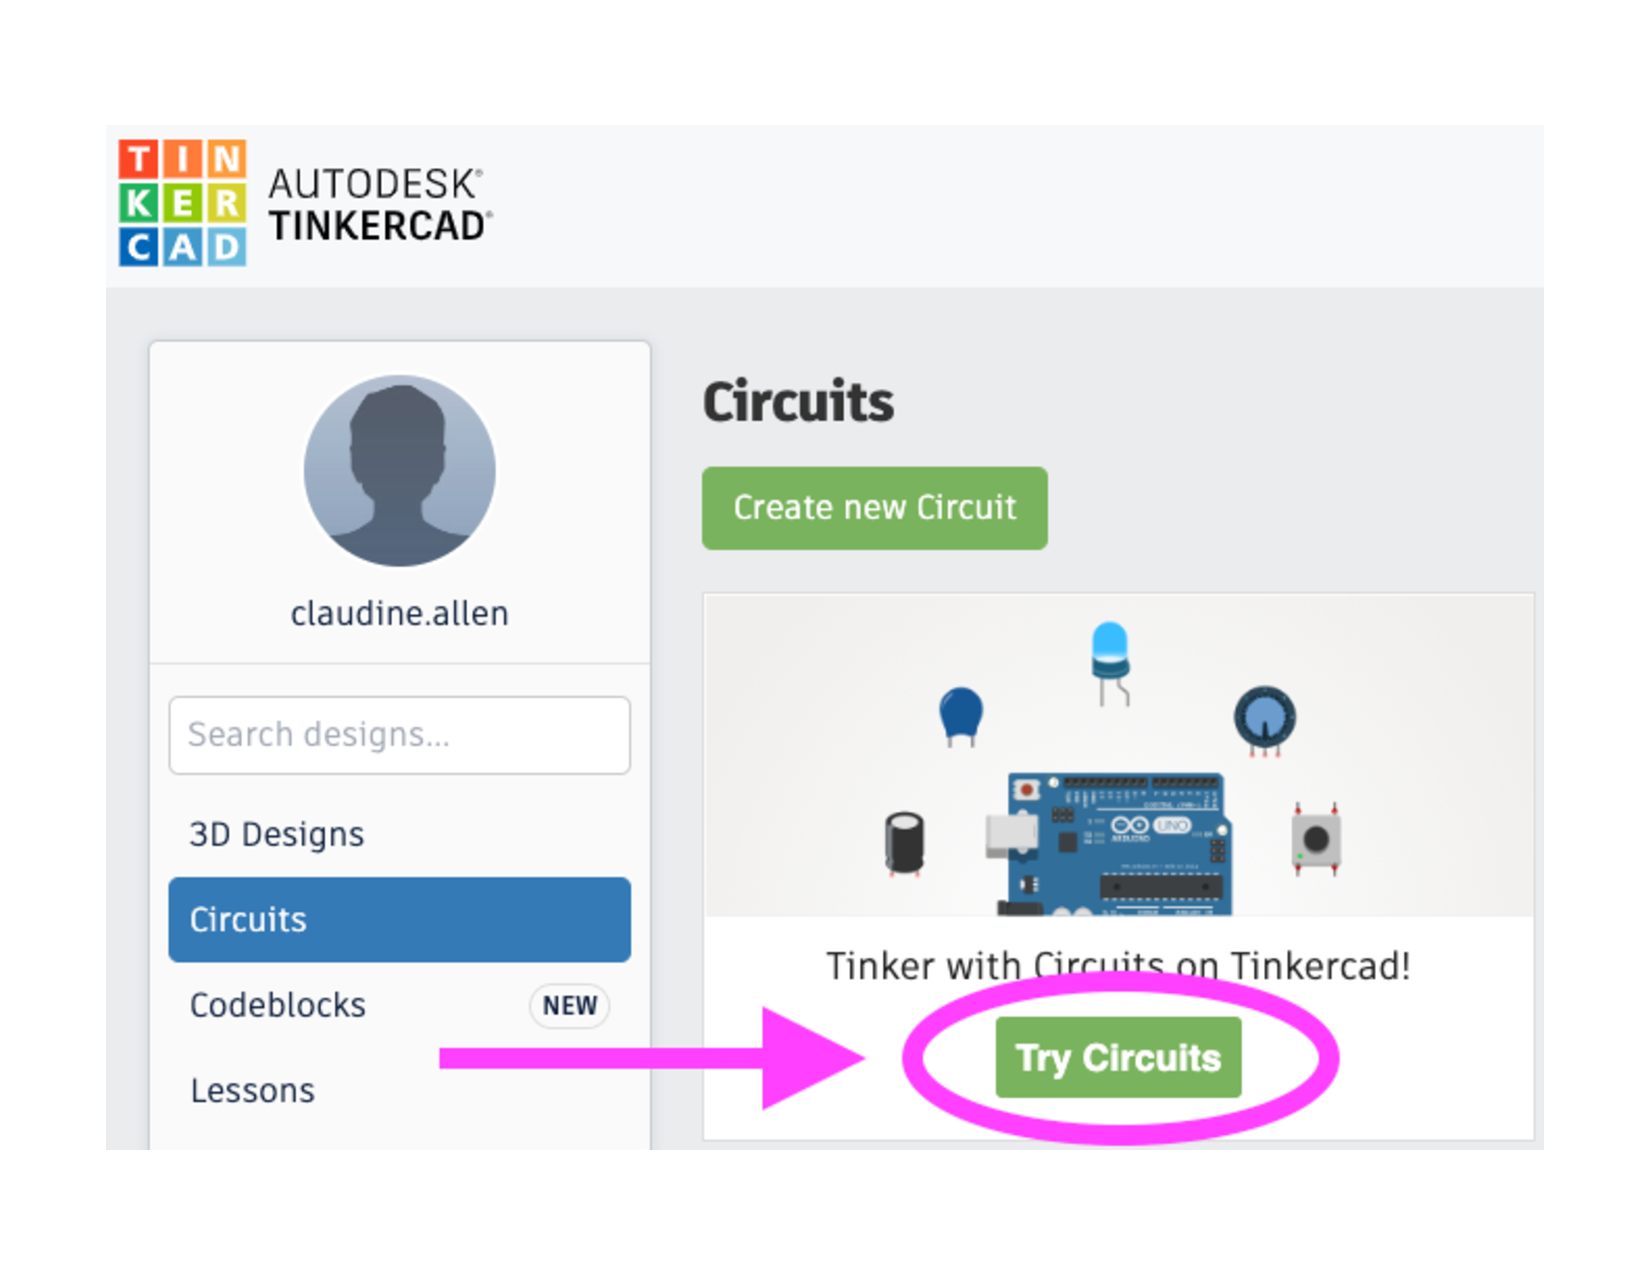
\includegraphics[width=.5\linewidth]{Tutoriel_Circuits_TinkerCad.pdf}
%     \caption{Capture d'écran du service infonuagique Tinkercad indiquant où trouver le tutoriel.}
%     \label{fig:tinkercad-trycircuits}
% \end{figure}

% Sur la gauche, vous trouverez la section \texttt{Circuits} rassemblant vos éventuels \texttt{Workspaces} de conception. À l'intérieur de ces derniers, vous pourrez aussi travailler sur vos designs de circuits en commun à l'aide du bouton \texttt{Share}.

% Complétez le tutoriel dans cette section, sans aucune note à prendre, en cliquant sur le bouton vert \texttt{Try Circuits} encerclé à la figure~\ref{fig:tinkercad-trycircuits}. Ce tutoriel est constitué de 4 leçons: \texttt{Start Simulating, Editing Components, Wiring Components} et \texttt{Adding Components}. Ce seront donc ces leçons qui seront évaluées individuellement, directement en ligne, pour ensuite faire virtuellement les manipulations du laboratoire sur Tinkercad lorsque vous êtes le.la membre de l'équipe en connexion à distance à la maison.
%Tinkercad et être la maison: mise à jour du 1er  protocole

%\newpage
\section[Matériel]{Matériel\footnote{Des photos accompagnent l'inventaire de composants \& instruments <\url{https://airtable.com/shrdI8Y6AqbNd7tZ8}> pour vous aider à identifier le matériel. Certains éléments, comme la patate(!), vous seront parfois remis au début du laboratoire.}} \label{sec:mat}

\noindent La réalisation de ce laboratoire requiert l'utilisation de:
\vspace{1ex}
\begin{itemize} \itemsep5pt
\item une pomme de terre;
\item un multimètre à 4\textonehalf~chiffres;
\item un multimètre à 6\textonehalf~chiffres;
\item un module d'acquisition (NI USB-6008);
\item un ordinateur avec le logiciel \textit{LabVIEW};
\item quatre tiges métalliques: acier, acier inoxydable\footnote{Pour la suite du document, pour éviter toute confusion avec l'acier, le terme «inox» sera utilisé pour désigner «acier inoxydable».}, aluminium et zinc;
\item deux résistances électriques (nominalement 12~$\Omega$ et 1~k$\Omega$);
\item une plaquette de montage (\textit{breadboard}).
\end{itemize}

\section{Manipulations} \label{sec:manip}

\setlength{\parskip}{1ex plus 0.5ex minus 0.2ex}

%\subsection{Partie 0 --- Exercice de statistiques en métrologie}

%Pendant la présentation introduisant des notions de base et un peu d'historique en métrologie, vous serez conviés à mesurer les dimensions d'une efface et estimer son volume avec 2 outils étalonnés. Ces mesures expérimentales seront rassemblées pour illustrer quelques concepts de statistiques et métrologie en fin de présentation.


\subsection{Partie 1 --- VI \textit{LabVIEW} contrôlant le module d'acquisition}

Tout au long de la création du VI \textit{LabVIEW}, n'oubliez pas d'enregistrer souvent votre fichier. À moins que vous ne teniez à tout recommencer du début\dots

a) Après vous être procuré le matériel complémentaire, soit une pomme de terre, quatre tiges et le module d'acquisition, branchez ce dernier dans un port USB de l'ordinateur.

b) Démarrez le logiciel \textit{LabVIEW} et ouvrez un VI vide. Faites \texttt{Ctrl+E} pour afficher le diagramme ainsi que la face-avant si une seule de ces deux interfaces est ouverte initialement. Le raccourci \texttt{Ctrl+H}, quant à lui, affiche une fenêtre d'aide contextuelle très utile.

c) Sur le diagramme, affichez la palette \textbf{Fonctions} à l'aide d'un clic droit et sélectionnez l'\textbf{Assistant DAQ} (\texttt{Fonctions $\rightarrow$ Express $\rightarrow$ Entrée $\rightarrow$ Assistant DAQ}). Placez l'Assistant DAQ sur le diagramme. Il se lancera automatiquement et la boîte de dialogue \textbf{Créer un nouvel objet Tâche Express} apparaîtra. Dans celle-ci, sélectionnez \texttt{Acquérir des signaux $\rightarrow$ Entrée analogique $\rightarrow$ Tension}. Sélectionnez la voie \textbf{ai0} et cliquez sur \textbf{Terminer}.

L'Assistant DAQ ouvrira ensuite une nouvelle boîte de dialogue qui affiche les options de configuration d'une boucle While pour la voie sélectionnée. Sous l'onglet \textbf{Configuration}, assurez-vous que les valeurs maximale et minimale de la gamme du signal d'entrée soient de 10~V et $-10$~V respectivement. Au bas de la page, changez le mode d'acquisition pour \textbf{Échantillons continus}, changez le nombre d'\textbf{Échantillons à lire} pour 10 et mettez une \textbf{Fréquence} de 10~Hz. Ceci signifie qu'à chaque itération le module acquerra 10~données et qu'il y aura 10~données prises à chaque seconde (donc une itération par seconde). Lorsque ceci est fait, cliquez sur \textbf{OK}. Une boîte de dialogue \textbf{Confirmer la création automatique de la boucle} apparaîtra. Cliquez sur \textbf{Oui} et \textit{LabVIEW} créera automatiquement une boucle While autour du VI.

Si vous avez correctement cliqué sur \textbf{Oui}, allez maintenant à l'étape c). Si vous avez cliqué sur \textbf{Non} (malheur!), vous devrez rajouter une boucle While manuellement. Pour ce faire, sélectionnez une boucle While (\texttt{Fonctions $\rightarrow$ Programmation $\rightarrow$ Structures $\rightarrow$ Boucle While}) et placez-la sur le diagramme de façon à ce qu'elle englobe l'Assistant DAQ (faites-la plus grande que nécessaire, d'autres objets devront être placés à l'intérieur de la boucle). Maintenant, rajoutez un bouton Stop. Pour ce faire, allez à la face-avant (\texttt{Ctrl+E}), ajoutez-y un bouton-poussoir (\texttt{Commandes $\rightarrow$ Moderne $\rightarrow$ Booléen $\rightarrow$ Bouton-poussoir}) puis changez son nom pour «stop~(F)». Par la suite, retournez au diagramme ; vous constaterez que le bouton Stop a été rajouté. Déplacez-le à l'intérieur de votre boucle While s'il n'y est pas déjà. Reliez la sortie du bouton Stop à l'entrée \textbf{stop~(F)} de l'Assistant DAQ et reliez la sortie \textbf{arrêtée} de l'Assistant DAQ au terminal de condition de la boucle While (l'octogone rouge). Vous pouvez agrandir l'icône de l'Assistant DAQ afin de mieux voir ses entrées et ses sorties.

d) Sur le diagramme, cliquez avec le bouton droit sur la sortie \textbf{Données} et sélectionnez \texttt{Créer $\rightarrow$ Indicateur graphe}. Un graphe apparaît sur la face-avant. Sur le diagramme, si l'indicateur graphe est placé à l'intérieur de la boucle While, celui-ci affichera les valeurs mesurées en continu. S'il est placé en-dehors de la boucle, alors il affichera l'ensemble des valeurs lorsque toutes les itérations auront été faites. Puisqu'on souhaite ce dernier type de graphique, placez l'indicateur en-dehors de la boucle (mais veillez à ce qu'il soit tout de même relié à l'aide d'un fil à la sortie \textbf{données} de l'Assistant DAQ).

e) Il serait intéressant d'avoir aussi un indicateur qui afficherait les valeurs mesurées pendant l'exécution du VI, pour voir si tout fonctionne correctement. Pour ce faire, encore sur la sortie \textbf{Données}, créez un indicateur numérique. Cet indicateur doit être placé dans la boucle pour avoir l'effet escompté.

f) Maintenant que le VI peut mesurer une tension et afficher les résultats en continu, il ne reste qu'à le configurer afin qu'il enregistre les résultats automatiquement dans un fichier sur l'ordinateur. Ajoutez la fonction \textbf{Écrire dans un fichier de mesures} (\texttt{Fonctions $\rightarrow$ Programmation $\rightarrow$ E/S sur fichiers $\rightarrow$} \texttt{Écrire dans un fichier de mesures}) et placez-le dans la boucle While, en bas à droite de l'Assistant DAQ (vous pouvez agrandir la boucle au besoin). La boîte de dialogue \textbf{Configurer Écrire dans un fichier de mesures} apparaît. Le champ \textbf{Nom de fichier} affiche l'endroit où les mesures seront enregistrées. Modifiez ce champ par un nom de fichier simple et représentatif en incluant la date. N'ayez pas peur de l'extension~\texttt{.lvm}: il s'agit d'un simple fichier texte.

Dans la section \textbf{Si le fichier existe déjà}, cochez l'option \textbf{Incrémenter le nom du fichier}. Dans la section \textbf{En-têtes de segment}, cochez \textbf{Un seul en-tête}. Cliquez sur \textbf{OK} lorsque tout est fait. Reliez la sortie \textbf{Données} de l'Assistant DAQ à l'entrée \textbf{Signaux} de l'icône Écrire dans un fichier de mesures.

g) Rajoutez maintenant un script qui arrêtera automatiquement le processus après 500 mesures. Pour ce faire, rajoutez une constante numérique (\texttt{Fonctions $\rightarrow$ Programmation $\rightarrow$ Numérique $\rightarrow$ Constante numérique}) et placez-la dans la boucle While, près du terminal d'itération (le carré bleu \textbf{i} représentant une variable qui contient la valeur de l'itération en cours). Fixez la constante à 50 (puisque 500 mesures correspondent à 50 itérations). Ensuite, insérez une commande de comparaison \textbf{Supérieur ou égal} (\texttt{Fonctions $\rightarrow$ Programmation $\rightarrow$ Comparaison $\rightarrow$ Supérieur ou égal~?}). Reliez le terminal d'itération \textbf{i} et la constante numérique aux entrées $x$ et $y$ respectivement de la fonction Supérieur ou égal, afin que le résultat soit faux lorsque $\mathbf{i}<constante$. Maintenant, supprimez le fil qui relie le bouton Stop à l'Assistant DAQ. Puis, reliez la sortie de la fonction Supérieur ou égal et la sortie du bouton Stop aux entrées d'une fonction \textbf{OU} (\texttt{Fonctions $\rightarrow$ Programmation $\rightarrow$ Booléen $\rightarrow$ OU}). Enfin, reliez la sortie du OU à l'entrée \textbf{stop~(F)} de l'Assistant DAQ. Ainsi, l'acquisition de données s'arrêtera lorsque 50 itérations auront été faites (soit 500 mesures) ou lorsque l'utilisateur appuiera sur le bouton Stop.

h) Le VI est maintenant terminé. Si ce n'était déjà fait, enregistrez-le! S'il vous reste des fils brisés, enlevez-les avec \texttt{Ctrl+B}, puis assurez-vous que votre VI soit le plus clair possible avec \texttt{Ctrl+U} et en déplaçant manuellement les fils et objets au besoin.


\subsection{Partie 2 --- Mesures de tension}

a) Insérez les tiges d'inox et d'aluminium dans la pomme de terre, de façon à avoir une distance de quelques centimètres entre les deux. Enfoncez-les bien. Faites attention de ne pas manger la patate ; cela viendrait fausser les résultats.

b) À l'aide du multimètre à 4\textonehalf~chiffres, mesurez la différence de potentiel entre les deux matériaux. Estimez très approximativement l'incertitude sur cette mesure, mais surtout justifiez-la en commentant brièvement comment vous êtes arrivés à cet estimé ainsi qu'en identifiant les causes de cette incertitude. 

c) Refaites la mesure avec le multimètre à 6\textonehalf~chiffres et notez l'incertitude en comparant à l'étape précédente.

d) Réalisez une acquisition de données informatiques avec le module d'acquisition. Pour ce faire, reliez les deux électrodes (les tiges d'inox et d'aluminium) aux bornes $+$ et $-$ de la voie \textbf{ai0}. À l'aide du VI que vous avez construit dans la première partie, faites l'acquisition des données puis transférez le fichier \texttt{.lvm} obtenu dans votre canal privé MS Teams via l'onglet correspondant accompagnant votre cahier de recherche. Notez que le crochet dans la fenêtre de transfert génère une publication et des notifications intempestives, à éviter svp. Vous pouvez aussi transférer tous vos fichiers pour le travail à distance seulement à la fin du laboratoire, mais n'oubliez pas de le faire, car l'ordinateur peut être réinstallé en effaçant les données à tout moment.
\vspace{1ex}

%%Une tcolorbox serait encore plus sympa pour ça :) :)
\noindent\framebox{\parbox{\dimexpr\linewidth-2\fboxsep-2\fboxrule}{\textbf{Sagesse expérimentale:} Toujours vérifier immédiatement que les données sont bien enregistrées dans votre fichier à l'aide d'un simple éditeur de texte, par exemple \textit{Bloc-notes (Notepad)} sur \textit{OS Windows} ou \textit{TextEdit} sur \textit{MacOS}. Un esprit critique attentif pourra même parfois déjà déceler des erreurs de mesures problématiques. Par exemple, une colonne entière de valeurs très proches de zéro peut être suspecte si le signal mesuré n'est pas censé être nul.}} 
\vspace{1ex}

e) Importez les données de votre fichier \texttt{.lvm} dans un format numérique à l'aide d'un des logiciels d'analyse suggérés dans le module de cours 2 de la section "Contenu et activités" sur le site Web\footnote{Le choix de logiciel n'est pas imposé à ce point-ci, mais il est recommandé d'évoluer progressivement vers les outils du langage \textit{Python} libre d'accès et bien adapté aux travaux de physique. L'équipe d'enseignement peut vous conseiller dans ce choix en fonction de votre niveau actuel de connaissances informatiques.} puis tracez leur graphique en nuage de points (\textit{scatter}). Vous constaterez que la résolution de l'appareil est très faible\footnote{N'hésitez pas à consulter l'équipe d'enseignement pour bien comprendre où la résolution intervient dans cette mesure.}. Pour améliorer la résolution de l'appareil, réduisez la gamme du signal d'entrée de l'Assistant DAQ : mettez des valeurs maximale et minimale de 1~V et $-1$~V respectivement. Puis, faites à nouveau une acquisition de données.

f) Construisez un histogramme à partir de vos nouvelles données : ajustez le nombre d'intervalles afin d'obtenir un histogramme significatif (trop ou trop peu d'intervalles ne permettent pas de bien voir la distribution des données).

g) Refaites les étapes a), d) et f) avec les combinaisons d'électrodes suivantes : acier--aluminium, aluminium--zinc et inox--zinc. Ne faites ces acquisitions que pour la gamme de valeurs réduite (de $-1$~V à $1$~V). Vous pouvez faire l'étape d'analyse en f) après le laboratoire si vous pensez manquer de temps. Observez que les fluctuations de la combinaison acier--aluminium permettent de mesurer la résolution de numérisation pour l'intervalle choisi.

h) Refaites les étapes d) et f) après avoir complètement débranché votre pomme de terre pour prendre une mesure de référence sur une gamme de valeurs encore plus réduite (de $-0.05$~V à $0.05$~V). Et oui, vous n’avez alors que le module d’acquisition de branché, sans rien d’autre! Retournez ensuite la plage de tension de $-0.5$~V à $0.5$~V pour les étapes subséquentes.

La plaquette de montage (\textit{breadboard}) simplifiera les branchements que vous aurez à faire pour la prochaine et dernière étape de l'expérience. Son utilisation est donc recommandée pour se familiariser avec son fonctionnent et deviendra essentielle dans les séances de laboratoire subséquentes.

i) Réinsérez les tiges d'inox et de zinc dans votre pomme de terre et connectez-les à l'entrée \textbf{ai0} du système d'acquisition. Rajoutez, en série, les deux résistances de 1~k$\Omega$ et de 12~$\Omega$ entre les deux matériaux (voir figure~\ref{L1-sch-patate}). Reliez les bornes de la petite résistance à l'entrée \textbf{ai1} du module d'acquisition. La mesure de la tension aux bornes de la petite résistance permettra de calculer le courant circulant entre les deux électrodes. Utilisez la plaquette de montage afin de faciliter les branchements de votre montage.

Modifiez votre VI afin qu'il puisse acquérir simultanément deux mesures de tension. Pour ce faire, allez dans les propriétés de l'Assistant DAQ et rajoutez une voie. Sélectionnez \textbf{Tension} puis \textbf{ai1} et faites \textbf{OK}. Laissez les mêmes paramètres que pour la voie \textbf{ai0} et cliquez sur \textbf{OK}. Sur le diagramme, mettez la valeur de la constante numérique à 10. Ainsi, les données seront recueillies pendant dix secondes au lieu de cinquante.

Maintenant, faites une acquisition des données. Sur votre logiciel d'analyse numérique choisi, divisez les valeurs de tension obtenues par la voie \textbf{ai1} par 12~$\Omega$ afin d'avoir le courant\footnote{Négligez l'incertitude de la résistance de 12~$\Omega$ pour ce calcul.} : ce courant est le même qui traverse la plus grosse résistance.

\begin{figure}[h]
\centering
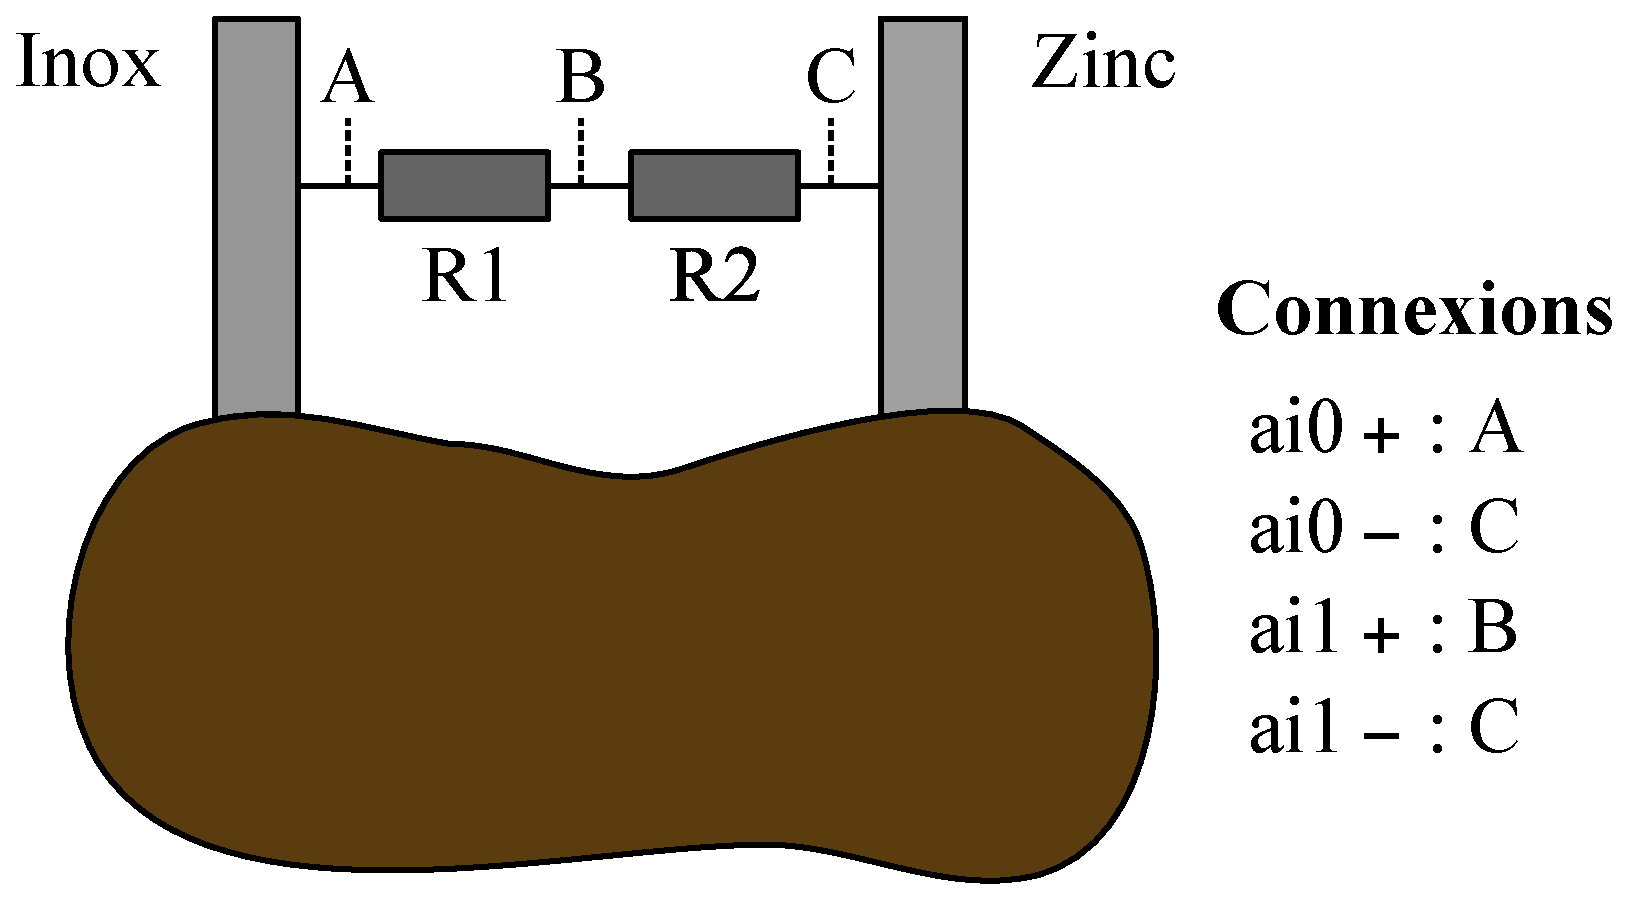
\includegraphics[width=0.6\textwidth]{L1-sch-patate}
\caption{\label{L1-sch-patate}Schéma du montage de la partie h) avec R1~=~1~k$\Omega$ et R2~=~12~$\Omega$.}
\end{figure}

\vspace{-0.5cm}
\section[Questions d'analyse I]{Questions d'analyse I\footnote{Pour cultiver de bonnes habitudes d'intégrité en recherche, les expériences échouées devront être reprises quitte à retourner au laboratoire VCH-0647 accessible en tout temps, soit exactement ce que vous feriez en milieu de travail professionnel. Les données et mesures d'autres équipes ne doivent donc pas être plagiées (professionnellement, ce serait alors une fraude scientifique) à moins d'une très rare autorisation du titulaire de cours; la provenance des données devra alors être explicitement citée pour éviter le plagiat. Pour compléter la sagesse expérimentale encadrée précédemment, il est alors clair que quelques vérifications préliminaires de vos données avant de quitter la séance de laboratoire, dans l'esprit d'arriver à bien répondre aux questions d'analyses, pourront vous éviter la perte de temps de recommencer des manipulations par la suite. Lorsque cela s'avère nécessaire malgré tout, votre technicien.ne du cours pourra sortir tout matériel qui n'est pas dans votre coffre le temps de votre travail puis le ranger; ses coordonnées de contact se retrouvent dans la section \texttt{Informations générales} sur la gauche du site de cours.}} \label{sec:grade} 

\vspace{-0.5cm}
\noindent$\rightarrow$ À remettre en équipe sur \href{https://www.gradescope.com/}{Gradescope} en ajoutant votre \href{https://help.gradescope.com/article/m5qz2xsnjy-student-add-group-members}{binôme de laboratoire} $\leftarrow$

\begin{gradescope}
\item Évaluez la résolution de numérisation (conversion analogique-numérique, échantillonnage) du module d'acquisition lors d'une mesure de tension pour les différents intervalles utilisés pendant le laboratoire, sachant que cette mesure est une différence (\textit{differential}) de potentiel entre deux points du circuit.\\ \textit{\footnotesize N.B. On fait appel à vos capacités de chercheur, dans le sens littéral de chercher par vous-même, pour comprendre le rôle du module d'acquisition avec son manuel et autres sources d'information (\emph{e.g.} dictionnaire!) sur la numérisation. Des discussions à ce sujet avec l'équipe d'enseignement et sur la chaîne de \texttt{Questions} du \texttt{Teams} de cours sont encouragées.}
    \begin{gradescope}
    \item Quelle est la résolution calculée pour l'intervalle de \qty{-10}{\volt} à \qty{10}{\volt}?
        \begin{itemize}[label=$\blacktriangleright$]
        \item \qty{4.9e-1}{\volt}
        \item \qty{4.9e-2}{\volt}
        \item \qty{4.9e-3}{\volt}
        \item \qty{4.9e-4}{\volt}
        \end{itemize}
    \item Quelle est la résolution calculée pour l'intervalle de \qty{-1}{\volt} à \qty{1}{\volt}?
        \begin{itemize}[label=$\blacktriangleright$]
        \item \qty{490}{\mV}
        \item \qty{49}{\mV}
        \item \qty{4.9}{\mV}
        \item \qty{0.49}{\mV}
        \end{itemize}
    \item Vous devriez observer un effet indésirable de cette limite de résolution dans au moins un de vos graphiques pour visualiser vos données. À laquelle des formes suivantes cela correspond-il le mieux? $\blacktriangleright$ Triangles $\blacktriangleright$ Rampes $\blacktriangleright$ Paliers %ou marches?
    \end{gradescope}
%\item À l'étape g) de la deuxième partie, vous avez probablement remarqué que la différence de potentiel entre les électrodes dépendait des métaux choisis. Quelle combinaison permet d'obtenir la plus haute tension?
    \begin{gradescope}
    \setcounter{gradescopei}{2}
    \item Avez-vous mesuré une tension qui fluctuait autour de zéro pour la combinaison acier--aluminium? $\blacktriangleright$ Oui $\blacktriangleright$ Non
    \item Si oui, pourquoi en est-il ainsi?
        \begin{itemize}[label=$\blacktriangleright$]
        \item L'acier est oxydé.
        \item Acier et aluminium commencent les deux par la lettre «a», donc ils ne peuvent réagir ensemble.
        \item Les deux métaux ont la même électronégativité.
        \end{itemize}
    \end{gradescope}
\item Comparez l’histogramme de l’étape~f) pour la combinaison inox-aluminium à celui de l’étape~h) en explicitant en légende lequel des deux correspond le mieux au modèle de la loi normale (distribution gaussienne). Pour le cas où cette loi ne s’applique PAS, présentez aussi graphiquement les données de tension d'une manière différente qui met en lumière le manque de stabilité de la mesure.
\item À partir des mesures de l'étape~i), calculez la valeur de la grosse résistance en utilisant une \textit{évaluation de Type A de l'incertitude} tel que présentée dans l’introduction aux bases de la métrologie. Concrètement, divisez la colonne \textit{tension} par la colonne \textit{courant} pour obtenir une distribution de la mesure de résistance. Puis, comparez la moyenne et la médiane de cette distribution de résistance.\\ \textit{N.B. Dans cette situation instable, il vaut mieux définir un intervalle d'incertitude très élargi en multipliant par 3 l'écart type~$\sigma$ de votre distribution de données.}
\item Laquelle ou lesquelles des questions précédentes peuvent être répondues en préparation avant le laboratoire? $\;\blacktriangleright$ Q1.1 $\;\blacktriangleright$ Q1.2 $\;\blacktriangleright$ Q1.3 $\;\blacktriangleright$ Q2.1 $\;\blacktriangleright$ Q2.2 $\;\blacktriangleright$ Q3 $\;\blacktriangleright$ Q4
\item \textsc{Sections de rapport - Introduction \& Conclusion:} Écrivez en moins de 350 mots (combinés) l'introduction et la conclusion d'un rapport scientifique portant sur l'ensemble du laboratoire.\footnote{Les instructions et explications d'écriture pour chaque section sont détaillées dans le document \texttt{Guide de rédaction de rapports scientifiques.}}
\end{gradescope}

\end{document}
OLLLDDDD STUFF!
%\footnote{Explication des \textit{tags} pour chaque numéro:\\
%\texttt{[observation]} : Réponse très courte ou à choix multiple visant à illustrer des commentaires que vous devez apprendre progressivement à remarquer et noter par vous-mêmes dans votre cahier pendant l'expérimentation pour développer votre jugement critique. Il faut réfléchir en manipulant! Cela aide à déceler des problèmes expérimentaux et ainsi développer le premier réflexe de tout chercheur.e et ingénieur.e, soit de modifier et reprendre l'expérience autant de fois que nécessaire.\\
%\texttt{[analyse]} : Résultats présentés selon les règles de présentation et d'écriture en métrologie. L'ensemble de votre réponse doit déjà faire preuve d'analyse critique dans cette étape préliminaire à la rédaction d'un rapport. Par exemple, si vos mesures et observations ont un comportement physiquement inattendu, une courte justification ou hypothèse doit être présentée pour tenter de l'expliquer. Une longue discussion n'est pas requise: la véracité et la qualité priment sur la quantité. Lorsqu'une figure ou un graphique est demandé, il doit respecter les consignes spécifiées dès le début de la page d'introduction du site Internet du cours.\\[-6pt]}